\section*{Appendix}

\begin{subappendices}
\section{Parameter Estimation}
\label{c3:appendix:A}
We estimate the parameters of the joint model using Markov chain Monte Carlo (MCMC) methods under the Bayesian framework. Let $\boldsymbol{\theta}$ denote the vector of all of the parameters of the joint model. The joint model postulates that given the random effects, the time to cancer progression, and the DRE and PSA measurements taken over time are all mutually independent. Under this assumption the posterior distribution of the parameters is given by:
\begin{align*}
p(\boldsymbol{\theta}, \boldsymbol{b} \mid \mathcal{D}_n) & \propto \prod_{i=1}^n p(l_i, r_i, \boldsymbol{y}_{di}, \boldsymbol{y}_{pi}, \mid \boldsymbol{b}_i, \boldsymbol{\theta}) p(\boldsymbol{b}_i \mid \boldsymbol{\theta}) p(\boldsymbol{\theta})\\
& \propto \prod_{i=1}^n p(l_i, r_i \mid \boldsymbol{b}_i, \boldsymbol{\theta}) p(\boldsymbol{y}_{di} \mid \boldsymbol{b}_i, \boldsymbol{\theta}) p(\boldsymbol{y}_{pi} \mid \boldsymbol{b}_i, \boldsymbol{\theta}) p(\boldsymbol{b}_i \mid \boldsymbol{\theta}) p(\boldsymbol{\theta}),\\
p(\boldsymbol{b}_i \mid \boldsymbol{\theta}) &= \frac{1}{\sqrt{(2 \pi)^q \text{det}(\boldsymbol{D})}} \exp(\boldsymbol{b}_i^T \boldsymbol{D}^{-1} \boldsymbol{b}_i),
\end{align*}
where, the likelihood contribution of the DRE outcome, conditional on the random effects is:
\begin{equation*}
p(\boldsymbol{y}_{di} \mid \boldsymbol{b}_i, \boldsymbol{\theta}) = \prod_{k=1}^{n_{di}} \frac{\exp\Big[-\mbox{logit} \big\{\mbox{Pr}(y_{dik} > \mbox{T1c})\big\} I(y_{dik}=\mbox{T1c}) \Big]}  {1+\exp\Big[-\mbox{logit} \big\{\mbox{Pr}(y_{dik} > \mbox{T1c})\big\}\Big]},
\end{equation*}
where $I(\cdot)$ is an indicator function which takes the value 1 if the $k$-th repeated DRE measurement ${y_{dik}=\mbox{T1c}}$, and takes the value 0 otherwise. The likelihood contribution of the PSA outcome, conditional on the random effects is:
\begin{equation*}
p(\boldsymbol{y}_{pi} \mid \boldsymbol{b}_i, \boldsymbol{\theta}) = \frac{1}{\big(\sqrt{2 \pi \sigma^2}\big)^{n_{pi}}} \exp\bigg(-\frac{{\lVert{\boldsymbol{y}_{pi} - \boldsymbol{m}_{pi}}\rVert}^2}{\sigma^2}\bigg),
\end{equation*}
The likelihood contribution of the time to cancer progression outcome is given by:
\begin{equation}
\label{c3:eq:likelihood_survival_part}
p(l_i,r_i\mid \boldsymbol{b}_i,\boldsymbol{\theta}) = \exp\Big\{-\int_0^{l_i} h_i(s)\mathrm{d}{s}\Big\} - \exp\Big\{-\int_0^{r_i}h_i(s)\mathrm{d}{s}\Big\}.
\end{equation}
The integral in (\ref{c3:eq:likelihood_survival_part}) does not have a closed-form solution, and therefore we use a 15-point Gauss-Kronrod quadrature rule to approximate it.

We use independent normal priors with zero mean and variance 100 for the fixed effects ${\{\beta_{0d},\ldots,\beta_{3d}, \beta_{0p},\ldots,\beta_{6p}\}}$, and inverse Gamma prior with shape and rate both equal to 0.01 for the parameter $\sigma^2$. For the variance-covariance matrix $\boldsymbol{D}$ of the random effects we take inverse Wishart prior with an identity scale matrix and degrees of freedom equal to 7 (number of random effects). For the relative risk model's parameters $\{\gamma_1, \gamma_2\}$ and the association parameters $\{\alpha_{1d}, \alpha_{1p}, \alpha_{2p}\}$, we use independent normal priors with zero mean and variance 100.

\subsection{Parameter Estimates}
\label{c3:appendix_subsec:A_paramestimates}
The longitudinal evolution of $\log_2 (\mbox{PSA} + 1)$ is modeled with non-linear terms, and hence the interpretation of the coefficients in this model is not straightforward. In the case of the evolution of DRE, the coefficients in the model correspond to a patient with a random effect value equal to 0. That is, the coefficients do not describe the marginal evolution of DRE over time. To avoid these issues, instead of the parameter estimates, in Figure~\ref{c3:fig:app1} and Figure~\ref{c3:fig:app2} we present the fitted marginal evolution of probability of $\mbox{DRE} > \mbox{T1c}$ and $\log_2 (\mbox{PSA} + 1)$, respectively, over a period of 10 years for a hypothetical patient who is included in AS at the age of 70 years. In addition, we present plots of observed versus fitted DRE and PSA profiles for nine randomly selected PRIAS patients in Figure~\ref{c3:fig:app3} and Figure~\ref{c3:fig:app4}, respectively. Lastly, the quantile-quantile plot of subject-specific residuals in Figure~\ref{c3:fig:app5} shows that the assumption of t-distributed (df=3) errors is reasonably met by the fitted model.

\begin{figure}
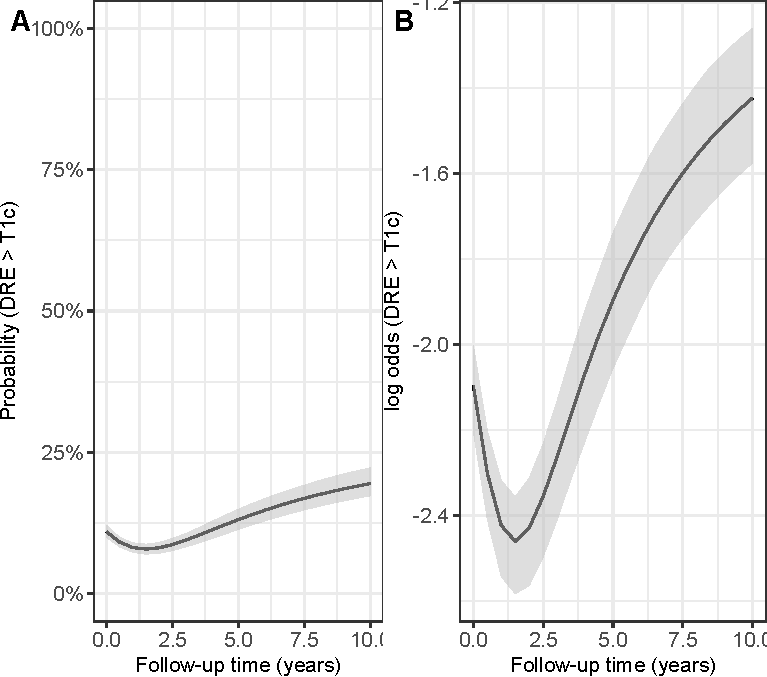
\includegraphics{contents/c3/images/c3_fig_app1.pdf}
\caption{\textbf{Fitted marginal evolution} of the probability of obtaining a DRE larger than T1c, and the corresponding marginal log odds, with 95\% credible interval. These results are for a hypothetical AS patient who is included in AS at the age of 70 years.}
\label{c3:fig:app1}
\end{figure}

\begin{figure}
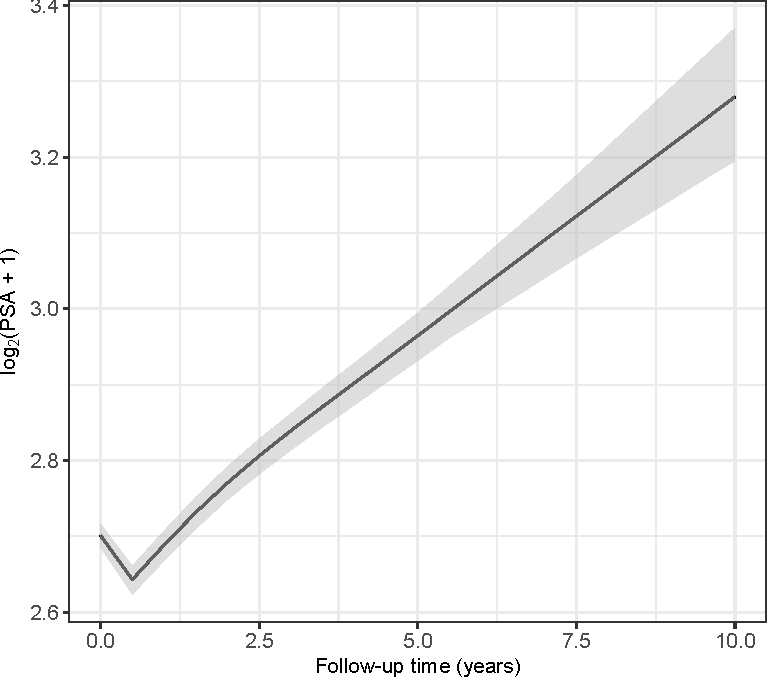
\includegraphics{contents/c3/images/c3_fig_app2.pdf}
\caption{\textbf{Fitted marginal evolution} of $\log_2(\mbox{PSA} + 1)$ measurements over a period of 10 years with 95\% credible interval, for a hypothetical patient who is included in AS at the age of 70 years.}
\label{c3:fig:app2}
\end{figure}

\begin{figure}
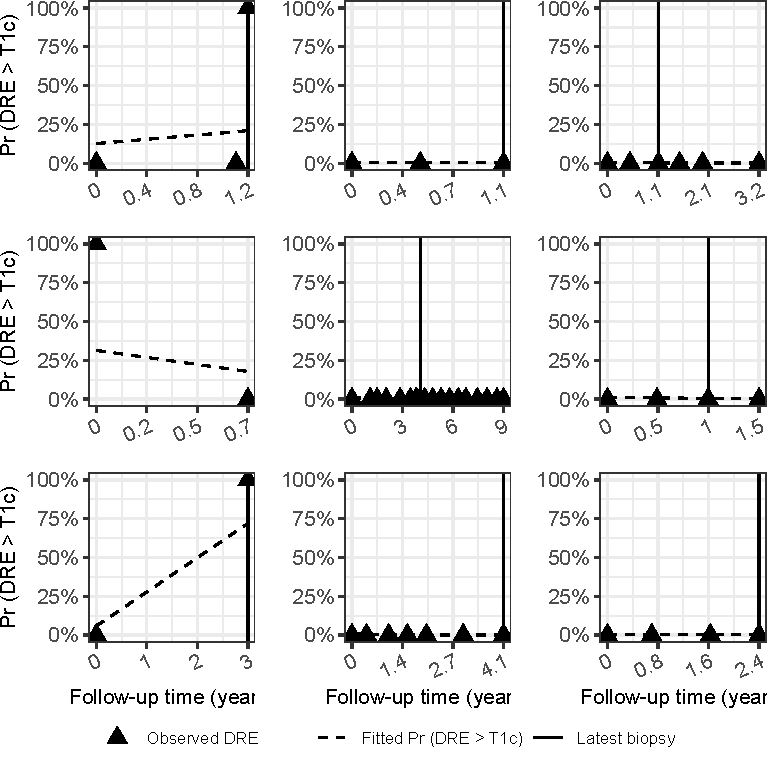
\includegraphics{contents/c3/images/c3_fig_app3.pdf}
\caption{\textbf{Observed DRE versus fitted probabilities} of obtaining a DRE measurement larger than T1c, for nine randomly selected PRIAS patients. The fitted profiles utilize information from the observed DRE measurements, PSA measurements, and time of the latest biopsy. Observed DRE measurements plotted against 0\% probability are equal to T1c. Observed DRE measurements plotted against 100\% probability are larger than T1c.}
\label{c3:fig:app3}
\end{figure}

\begin{figure}
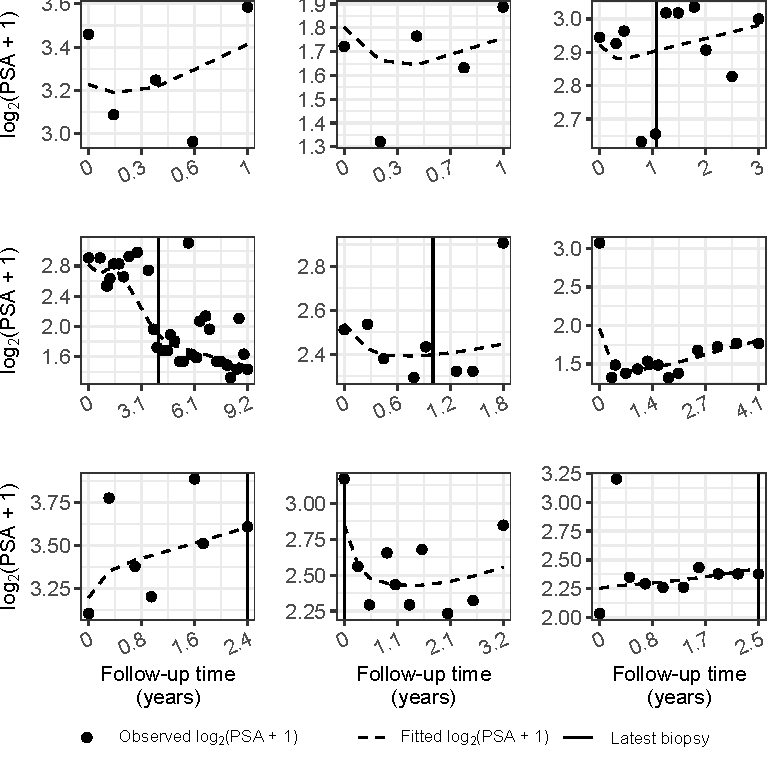
\includegraphics{contents/c3/images/c3_fig_app4.pdf}
\caption{\textbf{Fitted versus observed} ${\log_2(\mbox{PSA} + 1)}$ profiles for nine randomly selected PRIAS patients. The fitted profiles utilize information from the observed PSA measurements, DRE measurements, and time of the latest biopsy.}
\label{c3:fig:app4}
\end{figure}

\begin{figure}
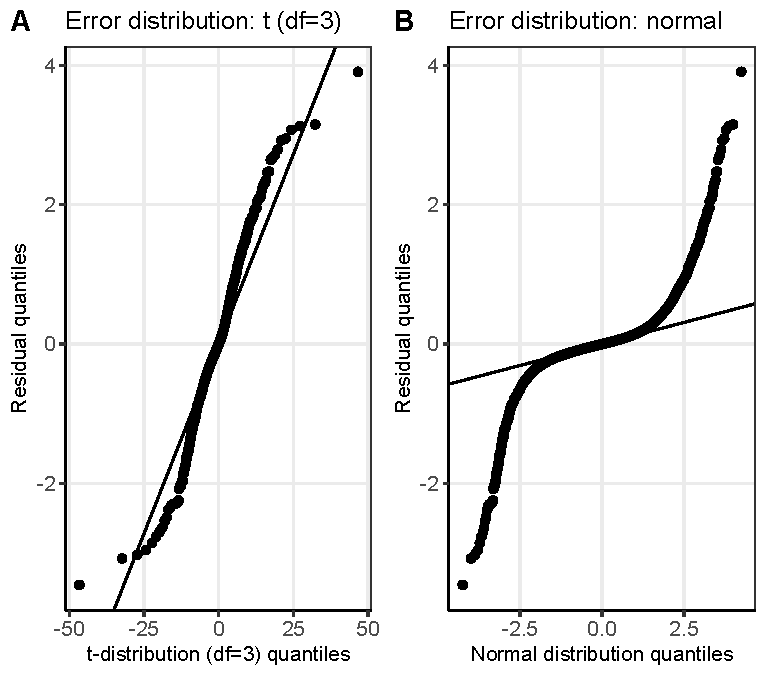
\includegraphics{contents/c3/images/c3_fig_app5.pdf}
\caption{\textbf{Quantile-quantile plot} of the subject-specific residuals from different joint models fitted to the PRIAS dataset. \textbf{Panel A}: model assuming a t-distribution (df=3) for the error term $\varepsilon_p$ \textbf{Panel B}: model assuming a normal distribution for the error term $\varepsilon_p$.}
\label{c3:fig:app5}
\end{figure}

For the relative risk sub-model, the parameter estimates in Table~\ref{c3:table:app1} show that both ${\log_2 (\mbox{PSA} + 1)}$ velocity, and the log odds of having ${\mbox{DRE} > \mbox{T1c}}$ were significantly associated with the hazard of cancer progression. It is important to note that since age, ${\log_2 (\mbox{PSA} + 1)}$ value and velocity, and log odds of ${\mbox{DRE} > \mbox{T1c}}$ are all measured on different scales, a comparison between the corresponding parameter estimates is not easy. To this end, in Table~\ref{c3:table:app2}, we present the hazard (of cancer progression) ratio, for an increase in the aforementioned variables from their first to the third quartile. For example, an increase in log odds of DRE > T1c, from -6.650 to -4.356 (fitted first and third quartiles) corresponds to a hazard ratio of 1.402. The interpretation of the rest is similar.

\begin{table}
\small
\centering
\caption{\textbf{Parameters of the relative-risk sub-model}: Estimated mean and 95\% credible interval. Age is median centered.}
\label{c3:table:app1}
\begin{tabular}{lrrrrr}
\toprule
Variable                      & Mean   & Std. Dev & 2.5\%  & 97.5\%                 & P              \\
\midrule
$(\mbox{Age} - 70)$                      & 0.012    & 0.006 & 0.000 & 0.022  & 0.045 \\
$(\mbox{Age} - 70)^2$ & -0.001   & 0.001 & -0.002 & 0.000      & 0.095 \\
$\mbox{logit} \big\{\mbox{Pr}(\mbox{DRE} > \mbox{T1c})\big\}$                 & 0.147    & 0.017 & 0.115  & 0.183  & \textless0.001     \\
Fitted $\log_2 (\mbox{PSA} + 1)$ value            & 0.104    & 0.078 & -0.044 & 0.256  & 0.193 \\
Fitted $\log_2 (\mbox{PSA} + 1)$ velocity             & 3.396    & 0.564 & 2.376  & 4.475  & \textless0.001   \\
\bottomrule
\end{tabular}
\end{table}

\begin{table}
\small
\centering
\caption{\textbf{Hazard (of cancer progression) ratio and 95\% credible interval (CI)}, for an increase in the variables of relative risk sub-model, from their first quartile ($\mbox{Q}_1$) to their third quartile ($\mbox{Q}_3$). Except for age, quartiles for all other variables are based on their fitted values obtained from the joint model fitted to the PRIAS dataset.}
\label{c3:table:app2}
\begin{tabular}{lrrr}
\toprule
Variable                      & $\mbox{Q}_1$   & $\mbox{Q}_3$ & Hazard ratio [95\% CI] \\
\midrule
Age & 65 & 75 & 1.129 [1.002, 1.251] \\
$\mbox{logit} \big\{\mbox{Pr}(\mbox{DRE} > \mbox{T1c})\big\}$ & -6.650 & -4.356 & 1.402 [1.301, 1.521]\\
$\log_2 (\mbox{PSA} + 1)$ value & 2.336 & 3.053 & 1.079 [0.969, 1.201]\\
$\log_2 (\mbox{PSA} + 1)$ velocity & -0.032 & 0.161 & 1.938 [1.582, 2.372]\\
\bottomrule
\end{tabular}
\end{table}

\subsection{Simulation Study Results}
In the simulation study, we evaluate the following in-practice fixed/heuristic approaches~\citep{loeb2014heterogeneity, inoue2018comparative} for biopsies: biopsy every year, biopsy every one and a half years, biopsy every two years and biopsy every three years. For the personalized biopsy approach, we evaluate three fixed risk thresholds: 5\%, 10\%, and 15\%, and a risk threshold was chosen using $\mbox{F}_1$ score. Lastly, we also evaluate the PRIAS schedule of biopsies. We compare all the aforementioned schedules on two criteria, namely the number of biopsies they schedule and the corresponding delay in detection of cancer progression in years (time of positive biopsy - the true time of cancer progression). The corresponding results, using ${\mbox{500} \times \mbox{250}}$ test patients are presented in Table~\ref{c3:table:app3}.

\begin{table}
\small
\centering
\caption{\textbf{Simulation study results for all patients}: Estimated first, second (median), and third quartiles for number of biopsies ($\mbox{Q}^{\mbox{nb}}_1$, $\mbox{Q}^{\mbox{nb}}_2$, $\mbox{Q}^{\mbox{nb}}_3$) and for the delay in detection of cancer progression ($\mbox{Q}^{\mbox{delay}}_1$, $\mbox{Q}^{\mbox{delay}}_2$, $\mbox{Q}^{\mbox{delay}}_3$), in years, for various biopsy schedules. The delay is equal to the difference between the time of the positive biopsy and the unobserved true time of progression. The results in the table are obtained from test patients of our simulation study.}
\label{c3:table:app3}
\begin{tabular}{l|rrr|rrr}
\toprule
In-practice schedules & $\mbox{Q}^{\mbox{nb}}_1$ & $\mbox{Q}^{\mbox{nb}}_2$ & $\mbox{Q}^{\mbox{nb}}_3$ & $\mbox{Q}^{\mbox{delay}}_1$  & $\mbox{Q}^{\mbox{delay}}_2$  & $\mbox{Q}^{\mbox{delay}}_3$ \\
\midrule
Every year (annual)         & 3  & 10 & 10 & 0.3 & 0.5 & 0.8 \\
Every 1.5 years      & 2  & 7  & 7  & 0.4 & 0.7 & 1.1 \\
Every 2 years       & 2  & 5  & 5  & 0.6 & 1.1 & 1.5 \\
Every 3 years      & 1  & 4  & 4  & 1.1 & 1.8 & 2.3 \\
PRIAS          & 2  & 4  & 6  & 0.3 & 0.7 & 1.0  \\
\midrule
\multicolumn{7}{l}{Personalized approach}\\
\midrule
Risk threshold: 5\%     & 2  & 6  & 8  & 0.3 & 0.6 & 0.9 \\
Risk threshold: 10\%    & 2  & 4  & 5  & 0.3 & 0.7 & 1.0   \\
Risk threshold: 15\%    & 2  & 3  & 4  & 0.4 & 0.8 & 1.4 \\
Risk using $\mbox{F}_1$ score & 1  & 2  & 3  & 0.5 & 0.9 & 2.2 \\
\bottomrule
\end{tabular}
\end{table}


\section{Source Code}
The source code for fitting the joint model is available at \url{https://github.com/anirudhtomer/prias/blob/master/src/chapter3_mdmpaper/fittingModel/jmFit.R}. 

The code generating the simulation population is available at \url{https://github.com/anirudhtomer/prias/blob/master/src/chapter3_mdmpaper/simulationStudy/controller.R}. 

The code for scheduling biopsies using fixed and risk based schedules is available at \url{https://github.com/anirudhtomer/prias/blob/master/src/chapter3_mdmpaper/simulationStudy/schedules.R}.

\end{subappendices}